\chapter{Experiments}

The goal of the experiments is two-fold:

\begin{itemize}
	\item Show that the traditional algorithms for $k$-center and $k$-median tend to produce unfair clusters

	\item Show that the proposed algorithm outputs clusters that respect the fairness guarantees
\end{itemize}


\section{Experiment Design}

3 datasets from \cite{Lichman2013} were used:
\begin{itemize}
	\item Diabetes (gender)
	\item Bank (married or not married)
	\item Sensus (gender)
\end{itemize}

The atttributes in the parenthesis are the protected attributes for each one. The unprotected attributes were chosen as the numeric attributes such as age, capital-gain...etc. (different for each dataset)

As for the algorithm, the flow-based fairlet decomposition algorithm (as discussed previously) was implemented.
For the vanilla $k$-center clustering algorithm, the {\it greedy furthest point algorithm\cite{Gonzalez1985}} was used.
For the vanilla $k$-median clustering algorithm, {\it single swap algorithm\cite{Arya2004}} was used. The reason for this choice, even though it obtains 5-approximation in the worst case, is that it performs well in practice. (Refer to Kanungo {\it et al.}, 2002) for more information.)

In all cases, the experiment was done with $t' = 2$ i.e. aiming for balance of at least $0.5$ in each cluster.

\newpage
\section{Results / Analysis}

\begin{figure}[hbt!]
\centering
  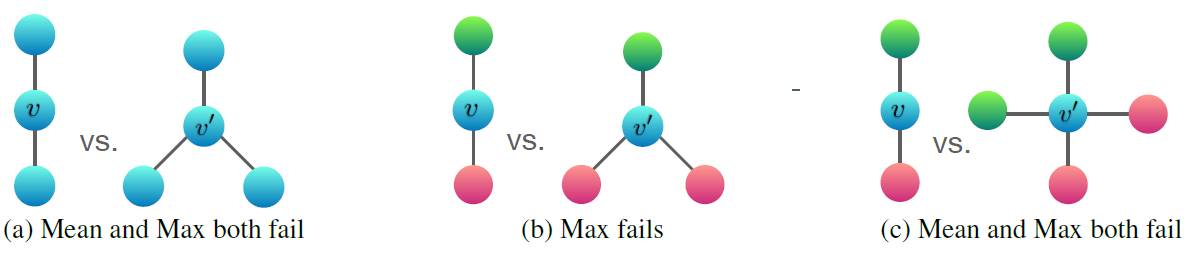
\includegraphics[height=7cm]{experiments/fig/fig4.png}
  \caption{Empirical performance of the classical and fair clustering median and center algorithms on the three datasets. The cost of each solution is on left axis, and its balance on the right axis.}
\end{figure}

Observe that as expected, the balance of the solutions produced by the classical algorithms is very low. More than half of the cases show the phenomenon of balance being at 0 for high value of $k$.

On the other hand the fair clustering solutions maintain a balanced solution, regardless of the value of $k$. Not surprisingly, the balance comes with a corresponding increase in cost, and the fair solutions are costlier than
their unfair counterparts.
In all of the scenarios the overall cost of the clustering converges
to the cost of the fairlet decomposition, which serves as a lower bound on the cost of the optimal solution.